\documentclass[10pt]{beamer}
\usetheme{AnnArbor}
\usecolortheme{default}
\graphicspath{ {./images/} }
\usepackage{cleveref}
\usepackage{hyperref}
\usepackage{listings}
\usepackage{multicol}

\definecolor{codegreen}{rgb}{0,0.6,0}
\definecolor{codegray}{rgb}{0.5,0.5,0.5}
\definecolor{codepurple}{rgb}{0.58,0,0.82}
\definecolor{backcolour}{rgb}{0.95,0.95,0.92}

\lstdefinestyle{mystyle}{
    backgroundcolor=\color{backcolour},   
    commentstyle=\color{codegreen},
    keywordstyle=\color{blue},
    numberstyle=\tiny\color{codegray},
    stringstyle=\color{codepurple},
    basicstyle=\ttfamily\footnotesize\footnotesize,
    breakatwhitespace=false,         
    breaklines=true,                 
    captionpos=b,                    
    keepspaces=true,                 
    numbers=left,                    
    numbersep=5pt,                  
    showspaces=false,                
    showstringspaces=false,
    showtabs=false,                  
    tabsize=2
}

\lstset{style=mystyle}

\setbeamertemplate{sections/subsections in toc}[square]
\setbeamertemplate{section in toc shaded}[default][100]
\setbeamertemplate{subsection in toc shaded}[default][100]
\setbeamertemplate{footline}{}
\setbeamertemplate{navigation symbols}{}
\setbeamertemplate{headline}{}
\setbeamertemplate{itemize items}[square]

\title{Eigenfaces, an application of SVD}
\author{Angelo Barbera}
\date{February 1, 2023}
\begin{document}


\begin{frame}
    \titlepage
\end{frame}


\begin{frame}
    \frametitle{Outline}
    \begin{multicols}{2}
      \tableofcontents
    \end{multicols}
    \end{frame}

\section{Eigenfaces}
\begin{frame}
    \frametitle{Eigenfaces}
    
    The \textit{eigenfaces} are a set of eigenvectors used in the problem of human face recognition. The method that makes use of
    eigenfaces for recognition was developed by Sirovich and Kirby in 1987. \vspace{4 pt}

    In order to compute eigenfaces it is necessary to flatten each image into a column vector and create a matrix using these vectors. \vspace{4 pt}
    
    Next we compute the mean of the matrix over the rows to calculate the "average face", and subtract the mean from each column to zero-mean center the data. \vspace{4 pt}
    
    Finally we can compute the Singular Value Decomposition of the data matrix obtaining the eigenvectors of the covariance matrix, which are also called eigenfaces. \vspace{4 pt}
    
    The eigenfaces express the directions of greatest variance and can be used to project the input data onto the space generated from the eigenvectors related to the directions of 
    greatest variance allowing to reduce the memory used to store the images.

\end{frame}

\section{Principal Component Analysis}
\begin{frame}
    \frametitle{Principal Component Analysis}
    
    The method previously described is based on Principal Component Analysis (PCA) that is a technique for reducing the dimensionality of a dataset. \vspace{4 pt}

    Given a set of data $ \{x_1, x_2, \dots, x_n \} $ where $ x_i \in \mathbb{R}^d $, we need to find a base of vectors $ W = \{w_1, \dots ,w_k \} $ where $ w_i \in \mathbb{R}^d $, such that the variance of 
    \begin{equation} y_1 = \begin{bmatrix} w_1^T x_1 \\ \vdots \\ w_k^T x_1 \end{bmatrix} , \dots, y_n = \begin{bmatrix} w_1^T x_n \\ \vdots \\ w_k^T x_n \end{bmatrix} \end{equation} is maximized. Considering the one dimensional case (k = 1) for semplicity, the variance is 
    \begin{equation} \sigma^2 = \label{eq:2} \frac{1}{n} \sum_{i=1}^{n} (w_1^T x_i- \mu)^2 \hspace{5 pt} \end{equation} 
    \begin{equation} \label{eq:3} \mu = \frac{1}{n} \sum_{i=1}^{n} w_1^T x_i = w_1^T \frac{1}{n} \sum_{i=1}^{n} x_i = w_i^T \overline x \end{equation} where $ \mu $ is the mean of the new coordinates and $ \overline x $ is the mean vector.
\end{frame}

\begin{frame}
    \frametitle{Principal Component Analysis}

    Substituiting \eqref{eq:3} into \eqref{eq:2} we get 

    \begin{gather} \nonumber \frac{1}{n} \sum_{i=1}^{n} (w_1^T x_i - w_1^T \overline x)^2 = \frac{1}{n} \sum_{i=1}^{n} (w_1^T (x_i - \overline x))^2 = 
        \\ \label{eq:4} = w_1^T \Bigg(\frac{1}{n} \sum_{i=1}^{n} (x_i - \overline x) (x_i - \overline x)^T\Bigg) w_1 = w_1^T C \hspace{1 pt} w_1 
    \end{gather}

    where $ C $ is the covariance matrix. To maximize \eqref{eq:4} we need to find the largest eigenvector of C in the one-dimensional case and the $ k $ largest eigenvectors $ W = \{w_1, \dots, w_k\} $ of C, in the k-dimensional case.
\end{frame}

\section{Singular Value Decomposition}
\begin{frame}
    \frametitle{Singular Value Decomposition}
    Given a matrix $ A \in \mathbb{R}^{m x n} $ it can be decomposed as 
    
    \begin{equation}
        A = U \Sigma V^T
    \end{equation}

    where $ U \in \mathbb{R}^{m x m} $ , $ V \in \mathbb{R}^{n x n} $ , $ \Sigma \in \mathbb{R}^{n x n} $ \vspace{3 pt}

    $ U $ and $ V $ are orthogonal matrices containing respectively the eigenvectors of $ A A^T $ (left singular vectors) and $ A^T A $ (right singular vectors). \vspace{5 pt}

    $ \Sigma $ is such that 

    \begin{equation}
        \Sigma_{ij} = \left\{
                \begin{array}{ll}
                    0 & i \neq j \\
                    \sigma_i & i = j
                \end{array}
            \right.
    \end{equation}

    \vspace{3 pt}

    where $ \sigma_1 \geq \sigma_2 \geq \cdots \geq \sigma_p \geq 0 $ , $ p = min(m, n) $ and $ \sigma_i = \sqrt{\lambda_i} $ where $ \lambda_i $ are the eigenvalues of $ A^T A $.
\end{frame}

\section{Computing Eigenfaces}
\begin{frame}
    \frametitle{Computing Eigenfaces}
    If the data are zero mean-centered, considering the k-dimensional case, we can rewrite \eqref{eq:4} as 
    \begin{equation}
        W^T (X X^T) W
    \end{equation} 

    therefore it is possible to calculate the k largest eigenvectors computing SVD of X
    
    \begin{equation}
        X = U \Sigma V^T 
    \end{equation} 

    where $ U $ contains the eigenvectors of $ X X^T $, and selecting only the first k left singular vectors. \vspace{5 pt}

    We can project new faces to the first k eigenfaces to store data using less memory in the following way
    
    \begin{equation}
        R = U_k^T X
    \end{equation}

    \vspace{5 pt}

    Where $ U_k $ is a $ d x k $ matrix containing the first k eigenfaces and $ X $ is a $ d x n $ matrix containing the flattened images, where $ n $ is the number of images and $ d $ is the height and width product of each image.
    The result is a $ k x n $ matrix with k $ \ll $ d.

\end{frame}

\section{Recovering Images}
\begin{frame}
    \frametitle{Recovering Images}
    We can recover original images using the k eigenfaces as a base for linear combinations of the reduced size images.
    
    Given $ U_K \in \mathbb{R}^{d x k} $ containing the first k eigenfaces, $ R \in \mathbb{R}^{k x n} $ containing the images projected into the space generated from the k eigenfaces, 
    and $ \bar X \in \mathbb{R}^{d x 1} $ containing the flattened mean face, let's recover an image as follows

    \begin{equation}
        I = U_K \textbf{r}_i + \bar X
    \end{equation}

    Where $ \textbf{r}_i $ is the i-th column vector of $ R $ corrisponding to the image to reconstruct. 
    Finally we have to reshape $ I $ as a matrix having the same dimensions of the original image in order to display the recovered image.
\end{frame}

\section{Implementation}
\begin{frame}
    \frametitle{Implementation}
    The following functions were used to implement the previously described algorithm and to analyze results:

    \begin{itemize}
        \item \textit{flatten} : returns the matrix $ X $ containing the flattened images.
        \item \textit{reduce} : returns the matrix $ U_K $ containing the first k eigenfaces, the matrix $ R $ containing the reduced images, the matrix $ M $ containing the mean face.
        \item \textit{recover\_image} : returns the recovered image from reduced data size.
        \item \textit{space\_used} : shows the space used to store the images as the captured information varies.
        \item \textit{eigenfaces\_used} : shows the eigenfaces used as the captured information varies.
    \end{itemize}
    
    The dataset used is "The ORL Database of Faces" created by AT\&T Laboratories Cambridge. This datased contains 400 images, the size of each image is 112 x 92 with 256 grey levels per pixel.

\end{frame}

\subsection{flatten}
\begin{frame}[fragile]
    \frametitle{flatten}
    
    \begin{lstlisting}[language=Matlab, numbers=none]
function [X] = flatten(image_path, n, height, width)
% Returns X given in input image_path, n, height, width.
% The name of the image must be "img (i)" where i is 
% the number of the image.
% The file extension of the image must be ".pgm".
% image_path is the path of the images. 
% n is the number of the images.
% height is the heigth of each image.
% width is the width of each image.
% X is the matrix containing the flattened images.
 
% dimension of each image
d = height*width;

% computing X
X = zeros(d,n);

for i=1:n
    filename = strcat(image_path, 'img (', num2str(i), ').pgm');
    image = imread(filename);
    image_double = im2double(image);
    X(:, i) = reshape(image_double, [d, 1]);
end
    \end{lstlisting}

\end{frame}

\subsection{reduce}
\begin{frame}[fragile]
    \frametitle{reduce}
   
    \begin{lstlisting}[language=Matlab, numbers=none]
function [U_K, R, M] = reduce(X, captured_info_tol)
% Returns the matrix U_K, R, M given in input X, height, width and
% captured_info_tol.
% X is the matrix containing the flattened images.
% captured_info_tol (between 0 and 1) is the desidered information
% to be captured.
% U_K is the matrix containing the first k eigenfaces.
% R is the matrix containing the flattened reduced images.
% M is the matrix containing the mean face.

% computing matrix M
M = mean(X, 2);

% zero mean centering of X
X_zero_mean = X - M;

% Singular Value Decomposition 
[U, S, ~] = svd(X_zero_mean, 'econ');
    \end{lstlisting}

\end{frame}

\begin{frame}[fragile]
    \frametitle{reduce}
   
    \begin{lstlisting}[language=Matlab, numbers=none]
% Selecting the number of eigenvectors to capture the 
% desidered information
S_diag = diag(S).^2;
captured_info = 0;
k = 1;
while(captured_info < captured_info_tol)
    captured_info = sum(S_diag(1:k)) / sum(S_diag);
    k = k + 1;
end

% selecting only the first k eigenvectors
U_K = U(:, 1:k);

% computing the reduced images
R = U_K' * X_zero_mean;  

    \end{lstlisting}

\end{frame}

\subsection{recover\_image}
\begin{frame}[fragile]
    \frametitle{recover\_image}

    \begin{lstlisting}[language=Matlab, numbers=none]
function [I] = recover_image(U_K, R, M, i, height, width)
% Returns the recovered image from reduced size data 
% given U_K, R, M, i, height, width.
% U_K is the matrix containing the first k eigenfaces.
% R is the matrix containing the flattened reduced images.
% M is the matrix containing the mean face.
% i is the index of the image to be recovered.
% height is the heigth of each image.
% width is the width of each image.
% I is the recovered image.

% recovering the flattened zero mean centered image
image_zero_mean = U_K * R(:, i);  

% adding mean faces to zero mean centered image
image_flattened = image_zero_mean + M;  

% reshaping the image to original size
I = reshape(image_flattened, [height, width]);

    \end{lstlisting}
    
\end{frame}

\subsection{space\_used}
\begin{frame}[fragile]
    \frametitle{space\_used}

    \begin{lstlisting}[language=Matlab, numbers=none]
function [x, y] = space_used(X)
% Returns the vectors relative to the memory used to 
% store the images as the captured information varies.
% X is the matrix containing the flattened images.
% x is the array containing the captured information.
% y is the array containing the saved space.

% initializing arrays
x = zeros(1, 9);
y = zeros(1, 9);

for i=1:1:9
    captured_info = i / 10;
    
    % reducing the images
    [U_K, R, M] = reduce(X, captured_info);
    
    % computing size of matrices
    size_X = size(X);
    size_R = size(R);
    size_U_K = size(U_K);
    size_M = length(M);
    \end{lstlisting}
    
\end{frame}


\begin{frame}[fragile]
    \frametitle{space\_used}

    \begin{lstlisting}[language=Matlab, numbers=none]
    % computing used space, reduced space and saved space
    original_used_space = size_X(1) * size_X(2);
    reduced_used_space = size_R(1) * size_R(2) + size_U_K(1) * size_U_K(2) + size_M;
    saved_space = round((1 - reduced_used_space / original_used_space) * 100);

    x(i) = round(captured_info * 100);
    y(i) = saved_space;

end

% plotting results
bar(x, y);
xlabel('Captured information (%)');
ylabel('Saved space (%)');
grid on

    \end{lstlisting}
    
\end{frame}

\subsection{eigenfaces\_used}
\begin{frame}[fragile]
    \frametitle{eigenfaces\_used}

    \begin{lstlisting}[language=Matlab, numbers=none]
function [x, y] = eigenfaces_used(X)
% Returns the vectors relative to the eigenfaces used 
% as the captured information varies.
% X is the matrix containing the flattened images.
% x is the array containing the captured information.
% y is the array containing the saved space.

% initializing arrays
x = zeros(1, 9);
y = zeros(1, 9);

for i=1:1:9
    captured_info = i / 10;
    
    % reducing the images
    [U_K, ~, ~] = reduce(X, captured_info);
    size_U_K = size(U_K);
    
    eigenfaces_used = size_U_K(2);

    x(i) = round(captured_info * 100);
    y(i) = eigenfaces_used;

end
    \end{lstlisting}
    
\end{frame}

\begin{frame}[fragile]
    \frametitle{eigenfaces\_used}

    \begin{lstlisting}[language=Matlab, numbers=none]
% plotting result
plot(x, y);
xlabel('Captured information (%)');
ylabel('Eigenfaces used');
grid on

    \end{lstlisting}
    
\end{frame}

\section{Results}

\subsection{Mean Face}
\begin{frame}
    \frametitle{Mean Face}
    The following image is the mean face, it is composed of the average features of the images in the dataset.

    \begin{center}
        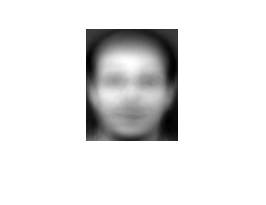
\includegraphics{mean_face}    
    \end{center}
    
\end{frame}

\subsection{Eigenfaces}
\begin{frame}
    \frametitle{Eigenfaces}
    The following images are the first 9 eigenfaces, they represent the main features of the images in the dataset.

    \begin{center}
        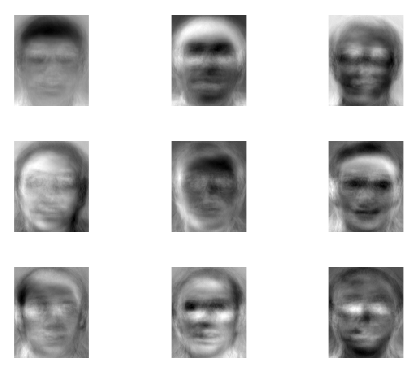
\includegraphics[scale=0.7]{first_9_eigenfaces}    
    \end{center}
    
\end{frame}

\subsection{Recovered image}
\begin{frame}
    \frametitle{Recovered image}
    The picture on the left is the original image, the picture on the right is the recovered image from reduced data with 90\% of captured information, the picture below is the recovered image from reduced data with 95\% of captured information.

    \begin{center}
        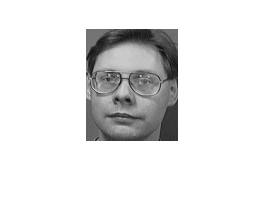
\includegraphics[scale=0.7]{original_image}
        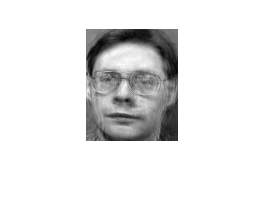
\includegraphics[scale=0.7]{recovered_0.9}    
        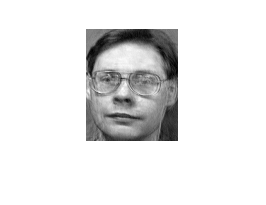
\includegraphics[scale=0.7]{recovered_0.95}
    \end{center}
    
\end{frame}

\subsection{Eigenfaces used}
\begin{frame}
    \frametitle{Eigenfaces used}
    The following image shows the eigenfaces used as the captured information varies.

    \begin{center}
        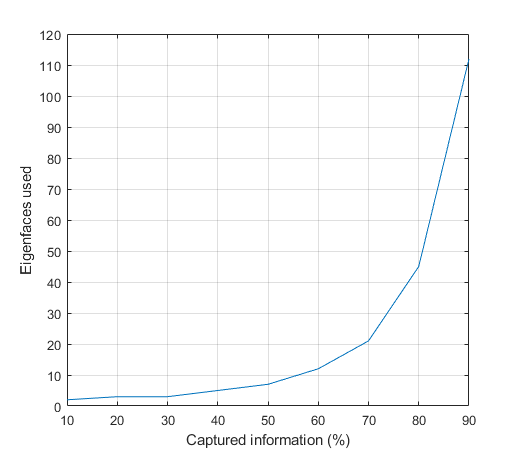
\includegraphics[scale=0.6]{eigenfaces_used}    
    \end{center}
    
\end{frame}

\subsection{Saved space}
\begin{frame}
    \frametitle{Saved space}
    The following image shows the saved space as the captured information varies.

    \begin{center}
        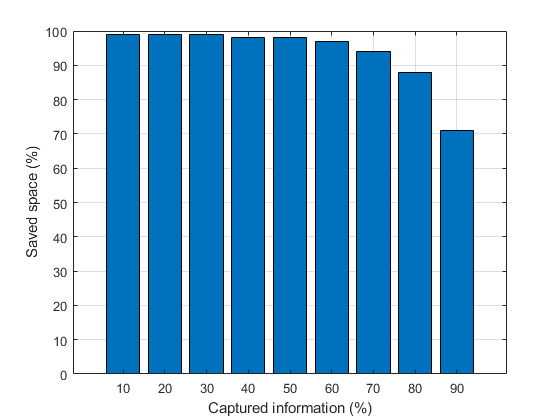
\includegraphics[scale=0.7]{space_used.png}    
    \end{center}
    
\end{frame}

\section{Face Recognition}
\begin{frame}
    \frametitle{Face Recognition}
    The face recognition can be implemented computing the matrices $ U_K $, $ R $, $ M $ using a training set and using an image belonging to a different set to recognize the image as a face belonging to the training set.
    
    Given the d x 1 vector $ i $ (corresponding to the flattened image having size h x w) and the matrices $ U_K $, $ R $, $ m $ (the flattened mean face), 
    it is possible to zero mean center $ i $ and project it into the space generated by the first k eigenfaces as follows
    
    \begin{equation}
        r = U_K^T (i - m)  
    \end{equation}

    To recognize the face we need to find the image $ l \in R $ that minimizes $ e = \lVert r - l \rVert_2 $ 

    Dataset of 99 images of 11 people, 9 image per person for training
    Dataset of 11 images of 11 people, 1 image per person for testing
\end{frame}

\section{Implementation}
\begin{frame}
    \frametitle{Implementation}
    The following functions were used to implement the algorithm : 

    \begin{itemize}
        \item flatten\_img : returns the vector $ img $ containing the flattened image
        \item reduce\_img : returns the vector $ r $ containing the flattened reduced image
        \item recognize\_img : returns the image found 
    \end{itemize}

    \vspace{5 pt}

    The training set is composed of 99 images of 11 people (9 images per person), while the testing set consists of 11 image (1 image per person).   
    The dataset used is extracted from ”The ORL Database of Faces” created by AT\&T Laboratories Cambridge.
    
\end{frame}

\subsection{flatten\_img}
    \begin{frame}[fragile]
        \frametitle{flatten\_img}

        \begin{lstlisting}[language=Matlab, numbers=none]
function [img] = flatten_img(image_path, i, height, width)
% Returns img given in input image_path, i, height, width.
% The name of the image must be "img (i)" where i is the 
% number of the image.
% The file extension of the image must be ".pgm".
% image_path is the path of the image 
% i is the number of the image
% height is the heigth of the image
% width is the width of the image
% img is the vector containing the flattened image
 
% image size
d = height*width;

% computing img
img = zeros(d, 1);

    filename = strcat(image_path, 'img (', num2str(i), ').pgm');
    image = imread(filename);
    image_double = im2double(image);
    img(:, 1) = reshape(image_double, [d, 1]);

        \end{lstlisting}
        
    \end{frame}

    \subsection{reduce\_img}
    \begin{frame}[fragile]
        \frametitle{reduce\_img}

        \begin{lstlisting}[language=Matlab, numbers=none]
function [r] = reduce_img(img, M, U_K)
% Returns the vector r given in input img, M, U_K.
% img is the vector containing the flattened image
% M is the matrix containing the mean face
% U_K is the matrix containing the first k eigenfaces
% r is the vector containing the flattened reduced image

% zero mean centering
img_zero_mean = img - M;

% computing the reduced image
r = U_K' * img_zero_mean;

        \end{lstlisting}
        
    \end{frame}

    \subsection{recognize\_img}
    \begin{frame}[fragile]
        \frametitle{recognize\_img}

        \begin{lstlisting}[language=Matlab, numbers=none]
function [img] = recognize_img(U_K, R, M, r, height, width)
% Returns img given in input U_K, R, M, r, height, width.
% U_K is the matrix containing the first k eigenfaces
% R is the matrix containing the flattened reduced images
% M is the matrix containing the mean face
% r is the image to be recognized
% height is the heigth of the image
% width is the width of the image.
% img is the image found

% searching the image
n = size(R, 2);
error = inf;
for i=1:n
    new_error = norm(r - R(:, i), 2);
    if new_error < error
        error = new_error;
        k = i;
    end 

    % recovering the image
    img = recover_image(U_K, R, M, k, height, width);
end
        \end{lstlisting}
        
    \end{frame}

\section{Results}
    \begin{frame}
        \frametitle{Results}
        The picture on the left is the image found, the picture on the right is the original image.
        \begin{center}
            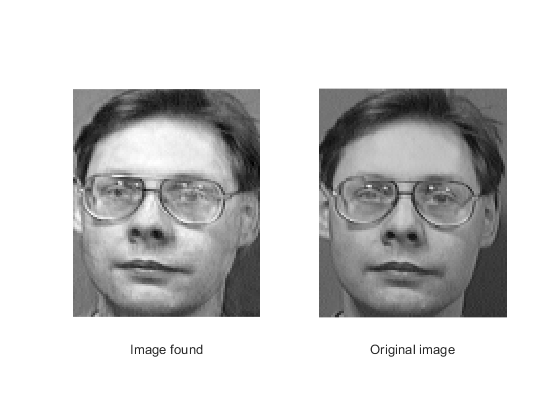
\includegraphics[scale=0.7]{recognized_face}    
        \end{center}
        
    \end{frame}

    \section{References}
\begin{frame}
    \frametitle{References}
    \begin{itemize}
        \item cs.nju.edu.cn/zlj/Course/DM\_16\_Lecture/Lecture\_2.pdf
        \item nextjournal.com/yuewangpl/svd-and-eigenfaces 
        \item cam-orl.co.uk/facedatabase.html 
        \item M. Turk and A. Pentland, "Eigenfaces for Recognition", Journal of Cognitive Neuroscience, vol.3, no. 1, pp. 71-86, 1991
    \end{itemize}
\end{frame}


\end{document}